\section{Демонстрация работы прототипа программного комплекса}

В целях исследования приминимости предложенного метода разработан прототип программного комплекса с ипсользованием СУБД Neo4j.

Демонстрация работоспособности прототипа программного комплекса выполнялось на сервере Ubuntu 20.04 (LTS) x64 со следующими характеристиками: 
\begin{itemize}
	\item 4 логических ядра;
	\item оперативная память 16~Gb;
	\item вторичная память 160~Gb.
\end{itemize}

База построена для параметра $k=8$, для 10 хромосом Arabidopsis thaliana, каждая из которых составляет от 18~млн до 30~млн символов. Размер базы составляет 65~548 узлов и 545~350 ребер.

В листинге \ref{lst:killme} представлен запрос на поиск вариантов последовательности нуклеотидов <<AAAAAAAGTGTCGTCGTCAAAAA>> в позиции $8$.

\begin{lstlisting}[label={lst:killme}, caption={Запрос на поиск вариантов последовательности нуклеотидов в заданной позиции.}]
WITH 8 as k, "AAAAAAAGTGTCGTCGTCAAAAA" as input, 8 as position
WITH  size(input) - k + 1 as kmerscnt, k, input, position
UNWIND range(position - k, position + k - 1) AS X
WITH left(right(input, kmerscnt + k - 1 - X), k) AS tmpkmer, kmerscnt, k
MATCH (selectedNode:KMer {value:tmpkmer})
WITH collect(selectedNode) as selectedNodes, k
WITH selectedNodes, selectedNodes[0] as head, last(selectedNodes) as tail, k
MATCH (s:Sequence)
MATCH (g:Genome)<-[:Belongs]-(s)
MATCH path=(head)-[:Precedes*(k-1)..(k+1)]->(tail) 
WHERE ALL(n in nodes(path) WHERE (n)-[:Belongs]->(s))
return {genome: g.name, sequence: s.name, variant: custom.pathToString(path), location: {start_kmer: ID(head), end_kmer: ID(tail)}};
\end{lstlisting}

В результате выполнения запроса в базе данных найдено 70 различных вариантов строки. Время выполнения запроса составило 5.7 секунд. Общий вид вывода приведен на рисунке \ref{fig:killme}.

\begin{figure*}[!th]
	\centering
	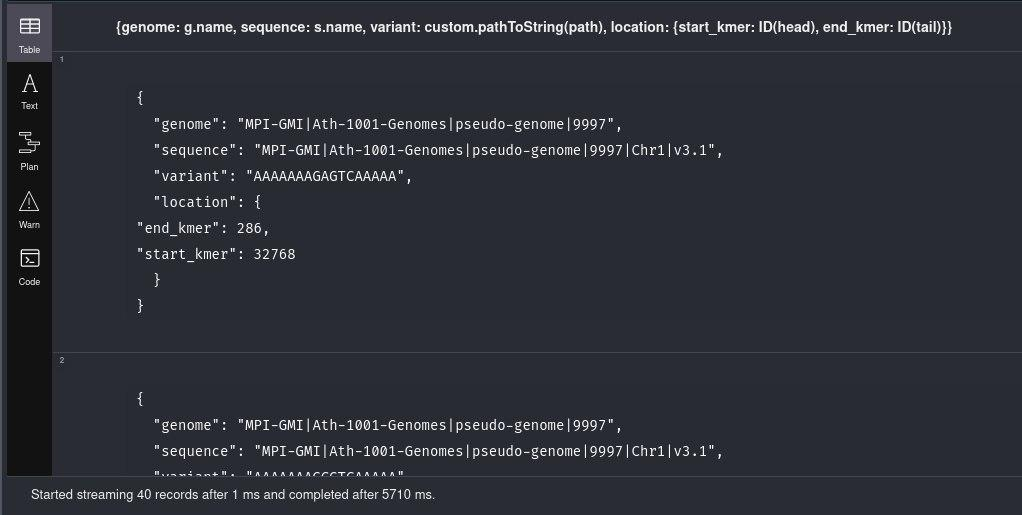
\includegraphics[width=0.8\textwidth]{img/killme.jpg}
	\caption{Результат выполнения запроса вариантов в клиенте базы данных Neo4j.}
	\label{fig:killme}
\end{figure*}

\pagebreak